\section{Dataset description}\label{sec:dataset_description}

As mentioned in Section~\ref{sec:data_collection}, the dataset contains
matrices \(A, B\) and \(R\) for a total of \(5,160,404\) parameter sets.
A descriptive analysis of the values of the parameters used in the experiments
is shown in Table~\ref{tab:parameters_descriptive}.


\begin{table}[H]
    \centering
    \caption{Descriptive statistics of the dataset}
    \begin{tabular}{|c|cccc|}
        \hline
        Parameter & Mean & Standard Deviation & Minimum & Maximum \\
        \hline
        \(\lambda_2\) & 4.545320 & 7.045888 & 0.100000 & 161.821844 \\
        \(\alpha\) & 0.504179 & 0.305070 & 0.000000 & 1.000000 \\
        \(t\) & 4.999915 & 3.036935 & 0.000000 & 10.000000 \\
        \hline
        \(\lambda_1^B\) & 1.217896 & 2.050153 & 0.000000 & 34.019111 \\
        \(\mu^A\) & 2.024239 & 0.400677 & 0.420571 & 6.773554 \\
        \(C^A\) & 1.081755 & 0.680075 & 1.000000 & 9.000000 \\
        \(N^A\) & 2.107661 & 0.821679 & 2.000000 & 24.000000 \\
        \(M^A\) & 2.045482 & 0.456713 & 1.000000 & 20.000000 \\
        \hline
        \(\lambda_1^A\) & 1.156440 & 2.628927 & 0.000000 & 60.961985 \\
        \(\mu^B\) & 2.052536 & 0.421094 & 2.000000 & 6.602015 \\
        \(C^B\) & 1.102124 & 0.784007 & 1.000000 & 9.000000 \\
        \(N^B\) & 2.121707 & 0.804273 & 2.000000 & 28.000000 \\
        \(M^B\) & 2.071752 & 0.560980 & 2.000000 & 16.000000 \\
        \hline
    \end{tabular}
    \label{tab:parameters_descriptive}
\end{table}


Not all values listed in Table~\ref{tab:parameters_descriptive} are used equally
often.
In fact consider the values of the parameter \(\lambda_2\) that range from
\(0.1\) to \(162\).
Figure~\ref{fig:data_description_lambda_2} shows the number of times each
value of \(\lambda_2\) is used in the dataset.

\begin{figure}[H]
    \centering
    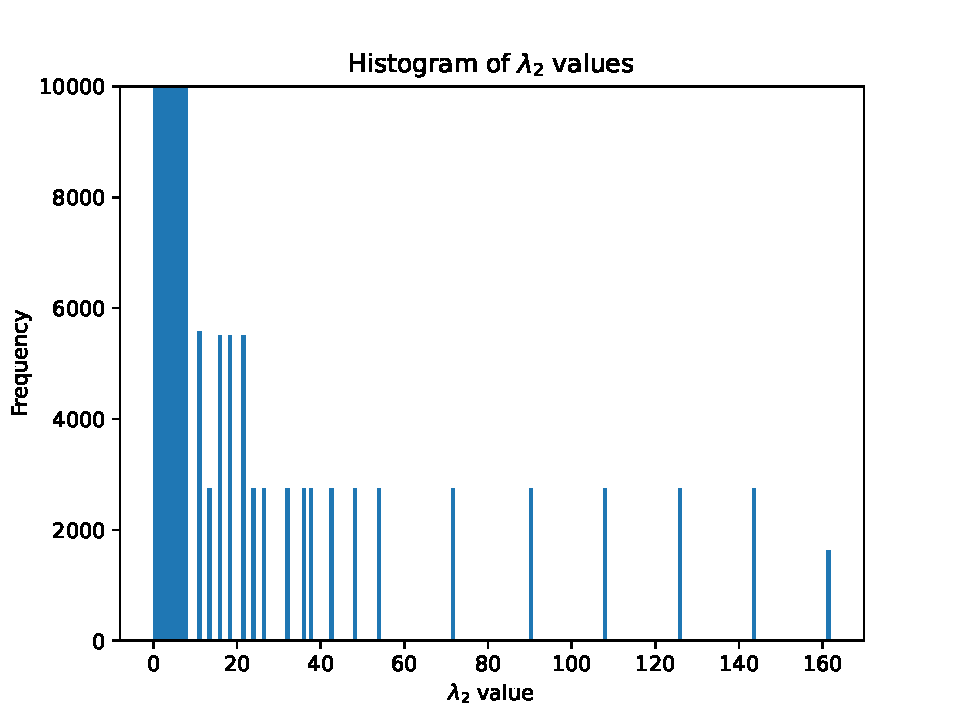
\includegraphics[width=\linewidth]{chapters/05_numerical_results/Bin/descriptive/lambda_2_histogram.pdf}
    \caption{Number of times each value of \(\lambda_2\) is used in the dataset}
    \label{fig:data_description_lambda_2}
\end{figure}

It can be seen that the values of \(\lambda_2\) that are used the most are
the ones from \(0.1\) to \(10\).
In fact, the y-axis of Figure~\ref{fig:data_description_lambda_2} has been cut
at \(10,\!000\) to better show the values of \(\lambda_2\) that are greater than
\(10\).
Figure~\ref{fig:data_description_lambda_2_0_10} shows the zoomed-in version of
Figure~\ref{fig:data_description_lambda_2} where only values of \(\lambda_2\)
from \(0\) to \(10\) are shown.
From Figures~\ref{fig:data_description_lambda_2}
and~\ref{fig:data_description_lambda_2_0_10} it can be seen that the values of
\(\lambda_2\) that are used the most are the ones from \(0\) to \(10\).

\begin{figure}[H]
    \centering
    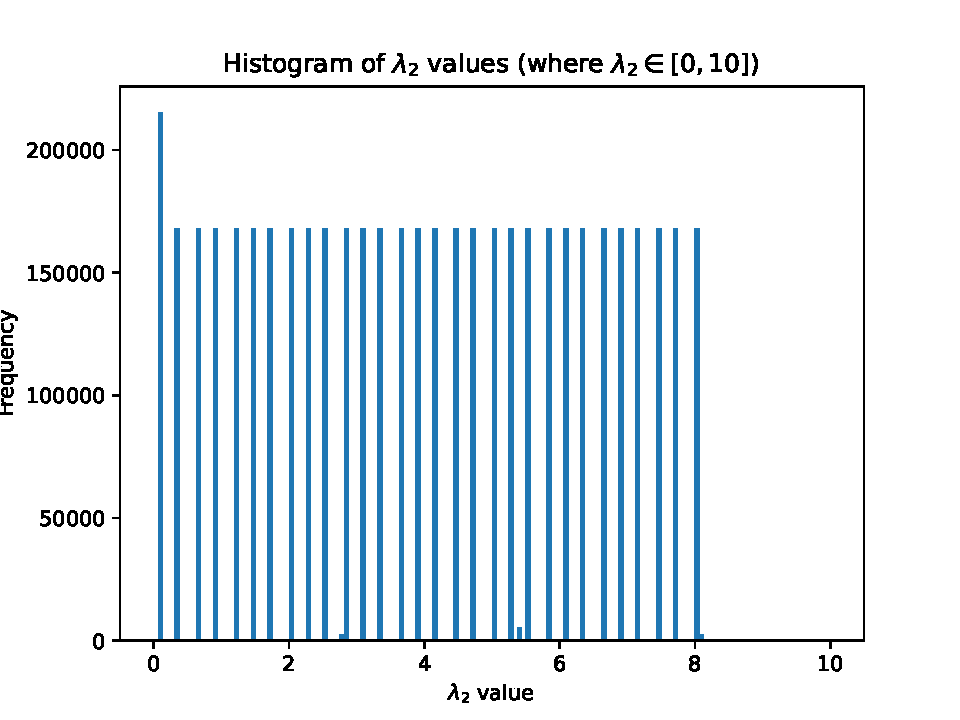
\includegraphics[width=\linewidth]{chapters/05_numerical_results/Bin/descriptive/lambda_2_histogram_0_10.pdf}
    \caption{Number of times each value of \(\lambda_2\) is used in the dataset
        for \(\lambda_2 \in [0, 10]\)}
    \label{fig:data_description_lambda_2_0_10}
\end{figure}

In addition, in terms of the values of \(C, N\) and \(M\) of the two players
\(A\) and \(B\), only some combinations of these values were explored.
Figures~\ref{fig:parameter_space_C_N_M_A} and~\ref{fig:parameter_space_C_N_M_B}
show the explored combinations of the values of \(C, N\) and \(M\) for player
\(A\) and player \(B\) respectively.

\begin{figure}[H]
    \centering
    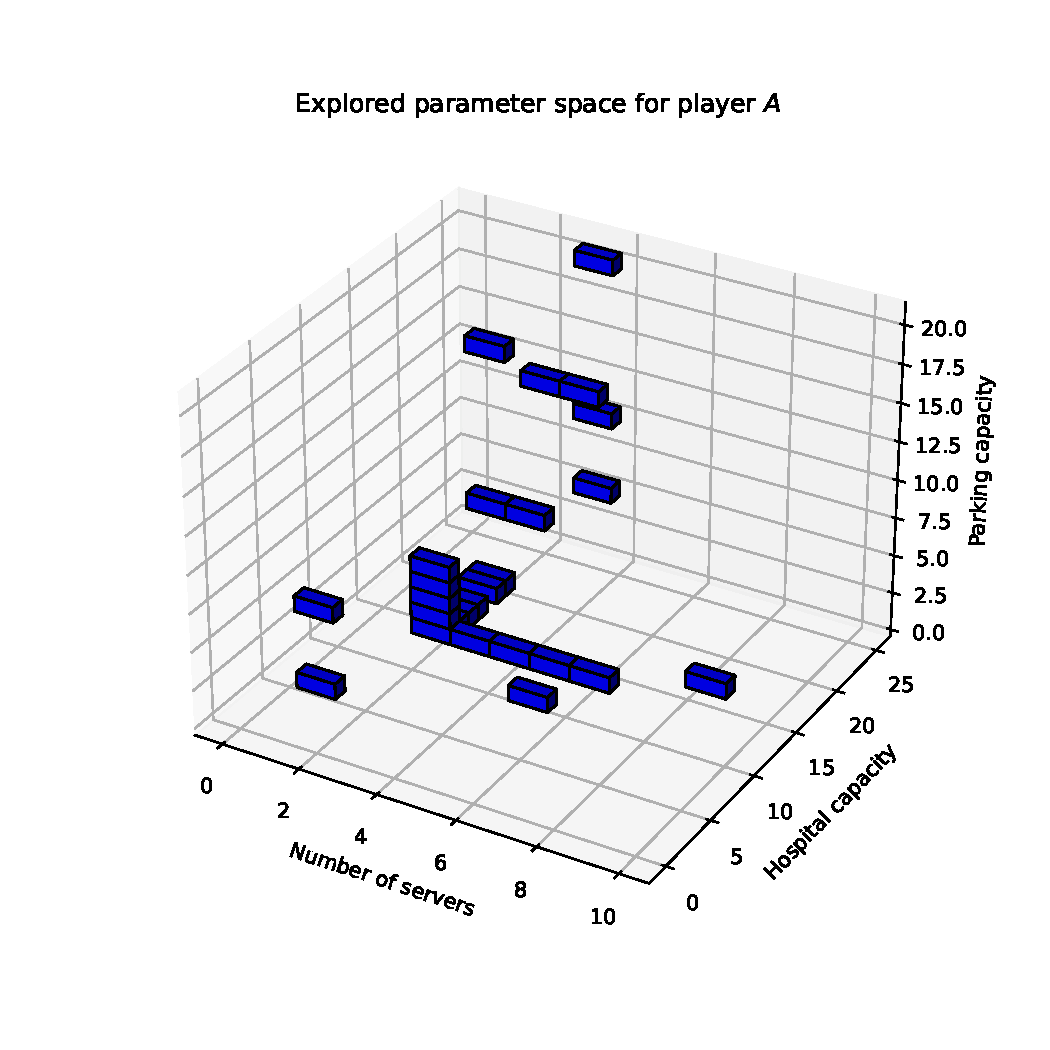
\includegraphics[width=\linewidth]{chapters/05_numerical_results/Bin/descriptive/explored_parameters_1.pdf}
    \caption{Explored combinations of the values of \(C, N\) and \(M\) for
    player \(A\)}
    \label{fig:parameter_space_C_N_M_A}
\end{figure}

\begin{figure}[H]
    \centering
    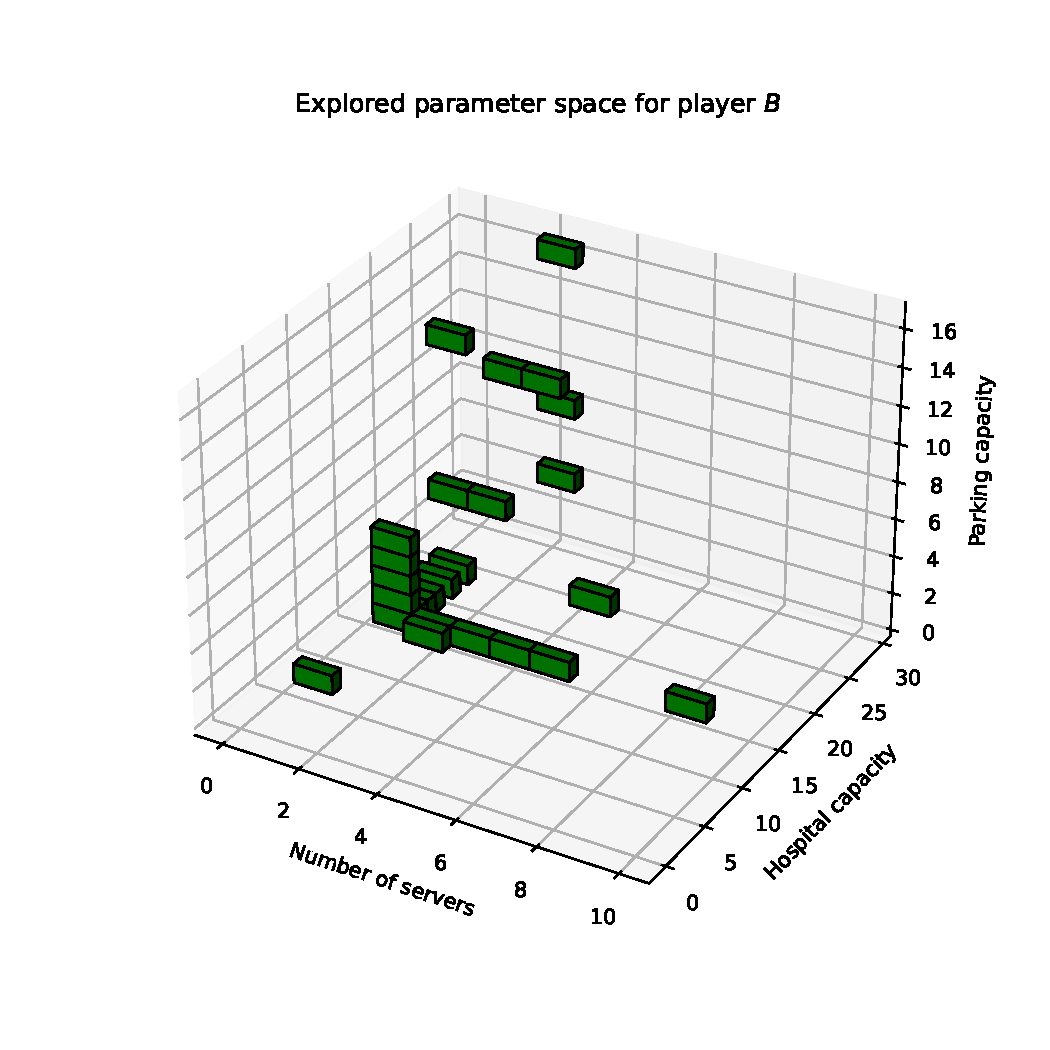
\includegraphics[width=\linewidth]{chapters/05_numerical_results/Bin/descriptive/explored_parameters_2.pdf}
    \caption{Explored combinations of the values of \(C, N\) and \(M\) for
    player \(B\)}
    \label{fig:parameter_space_C_N_M_B}
\end{figure}

From Figures~\ref{fig:parameter_space_C_N_M_A}
and~\ref{fig:parameter_space_C_N_M_B} it can be seen that only a small subset
of the possible combinations of the values of \(C, N\) and \(M\) were explored.
Note here that for each of this explored combinations additional combinations
of the values of \(\lambda_2, \lambda_1^A, \lambda_1^B, \mu^A, \mu^B, \alpha\)
and \(t\) were also used.

